%=======================02-713 LaTeX template, following the 15-210 template==================
%
% You don't need to this template
%
\documentclass[11pt]{article}
\usepackage{amsmath,amssymb,amsthm}
\usepackage{graphicx}
\usepackage[margin=1in]{geometry}
\usepackage{fancyhdr}
\usepackage{multicol}
\setlength{\parindent}{0pt}
\setlength{\parskip}{5pt plus 1pt}
\setlength{\headheight}{13.6pt}
\newcommand\tab[1][1cm]{\hspace*{#1}}
\newcommand\question[2]{\vspace{.25in}\hrule\textbf{#1: #2}\vspace{.5em}\hrule\vspace{.10in}}
\renewcommand\part[1]{\vspace{.10in}\textbf{(#1)}}
\newcommand\header[4]{\begin{center}{#1} \\ {#2} \\ {#3} \\ \textbf{#4} \end{center}}

\begin{document}\raggedright

\header
	{ITU Computer and Informatics Faculty}
	{BLG 454E Learning From Data, Spring 2018}
	{Homework \#4}
	{Due May 27, 2018 11pm}

\begin{center}
	Kadir Emre Oto \\
	(150140032)
\end{center}

\question{1}{Multilayer Perceptron}

\part{a} (25 pts) Report cross entropy error value for 1, 2, 3, 4, 5, 6, 7, 8, 9, 10, 50, 100, 200th iteration in the backpropagation(training) phase.

According the results which is given below, if iteration count is incresed, the accuracy increases and the cross entropy error value decreases.

\begin{multicols}{2}
Iteration Count: 1 \\
Cross Entropy Error: 5560.259742484045 \\
Accuracy: 0.75 \\
----------  \\
Iteration Count: 2 \\
Cross Entropy Error: 2455.591097218306 \\
Accuracy: 0.8333333333333334 \\
---------- \\
Iteration Count: 3 \\
Cross Entropy Error: 1553.4939942454293\\
Accuracy: 0.9166666666666666\\
----------\\
Iteration Count: 4\\
Cross Entropy Error: 1430.0461926499293\\
Accuracy: 0.8333333333333334\\
----------\\
Iteration Count: 5\\
Cross Entropy Error: 1923.7371876472791\\
Accuracy: 0.75\\
----------\\
Iteration Count: 6\\
Cross Entropy Error: 1077.1906751938932\\
Accuracy: 0.8333333333333334\\
----------\\
Iteration Count: 7\\
Cross Entropy Error: 1059.2269895314132\\
Accuracy: 0.8333333333333334\\
----------\\
Iteration Count: 8\\
Cross Entropy Error: 968.299161454117\\
Accuracy: 0.9166666666666666\\
----------\\
Iteration Count: 9\\
Cross Entropy Error: 1005.9774139521438\\
Accuracy: 0.8333333333333334\\
----------\\
Iteration Count: 10\\
Cross Entropy Error: 775.3261478428205\\
Accuracy: 0.8333333333333334\\
----------\\
Iteration Count: 50\\
Cross Entropy Error: 437.0891897898743\\
Accuracy: 0.8333333333333334\\
----------\\
Iteration Count: 100\\
Cross Entropy Error: 280.4186414102801\\
Accuracy: 1.0\\
----------\\
Iteration Count: 150\\
Cross Entropy Error: 281.14420842642227\\
Accuracy: 0.9166666666666666\\
----------\\
Iteration Count: 200\\
Cross Entropy Error: 196.63660369996987\\
Accuracy: 0.9166666666666666\\
\end{multicols}

\cleardoublepage

\part{b} (25pts)Use trained multilayer perceptron model and calculate the accuracy for test set(dataTest.csv) and report it.

The accuracy valus for test dataset is also given at \textbf{part a} for different iteration count. Average accuracy is higher than 90 percent. After 200 iterations, the accuracy may be 100 percent as Figure 1.

\begin{figure}[h]
	\centering
	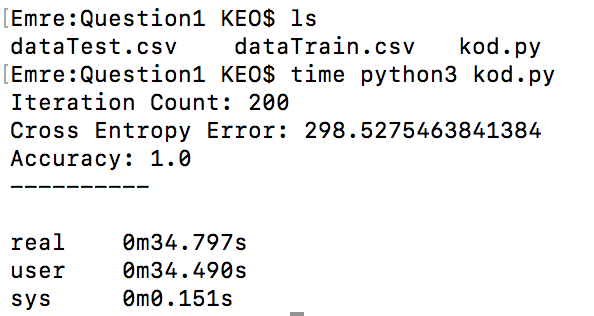
\includegraphics[width=0.6\linewidth]{q1_result}
	\caption{Example usage of program and the result}
	\label{fig:q1_result}
\end{figure}

\question{2}{Clustering}

\textbf{In this question, the first field of the data is discarded because the label of the field is not determined!}

\part{a} Calculate Sum of Squared Error(SSE) value for k=1, 5, 10 and 20 in this dataset and report them. Decide which k value is the best clustering parameter for this dataset and report it.

According to the results, the SSE value decreases while k value increases.

\begin{figure}[h]
	\centering
	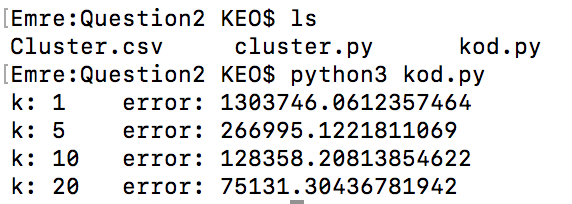
\includegraphics[width=0.6\linewidth]{sum_of_squared_error}
	\caption{Example usage of program and the results}
	\label{fig:sum_of_squared_error}
\end{figure}

\cleardoublepage

\part{b} (25 pts) Cluster this dataset using finded the best k value in section a. Draw the decision boundaries and report it.

I choose the k value as 20, because its sum of squared error is lowest. 

\begin{figure}[h]
	\centering
	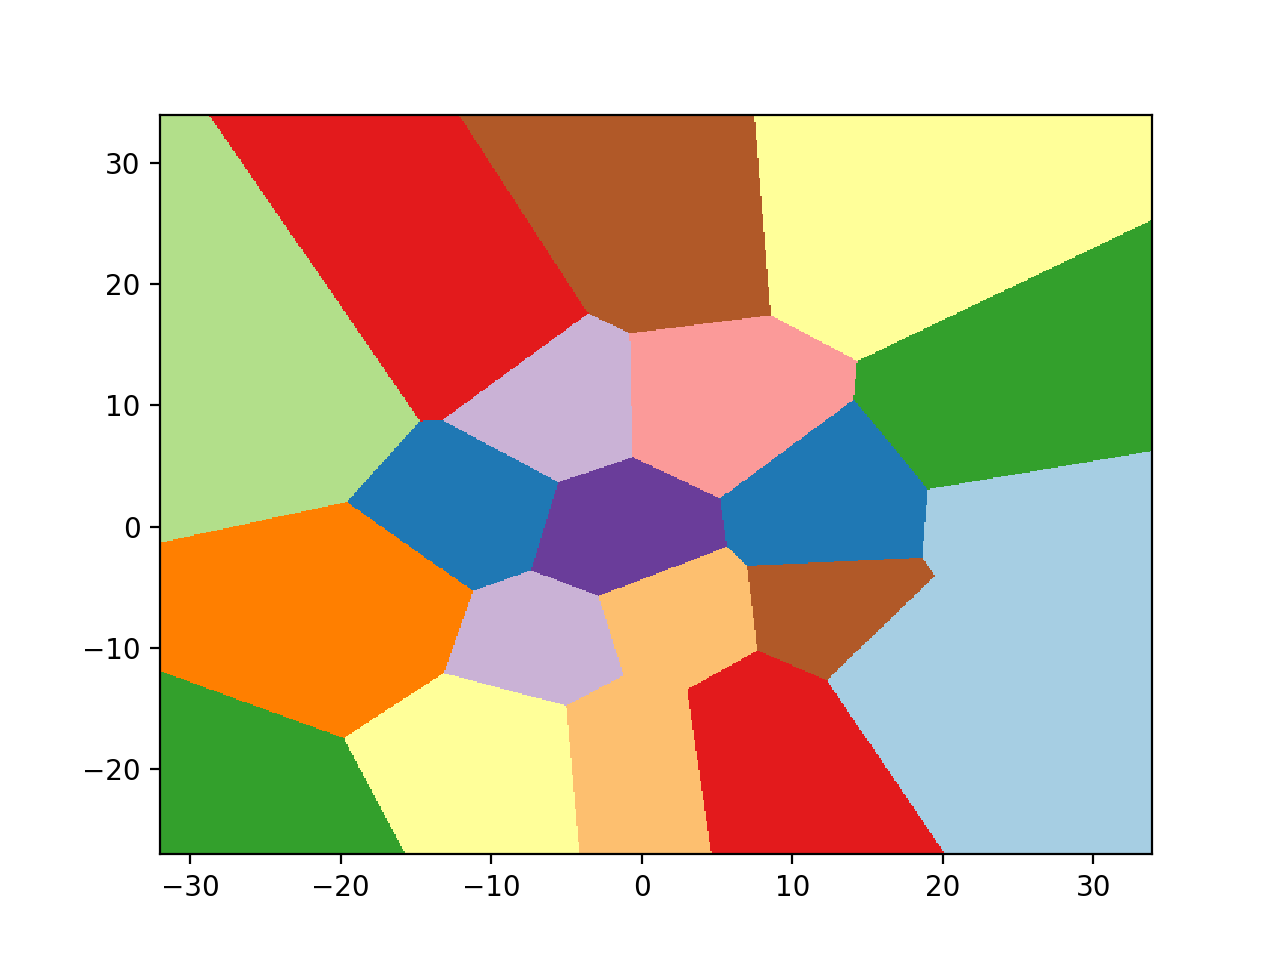
\includegraphics[width=0.6\linewidth]{decision_boundaries}
	\caption{The decision boundaries}
	\label{fig:decision_boundaries}
\end{figure}

\end{document}
